\subsection{User Study}~\label{exp:user_study}

We conducted a Wizard-of-Oz (WoZ) user study to evaluate how different query policies affect user performance, interaction cost, workload, and situation awareness. While the system evaluation in Section~\ref{exp:sys_eval} measures autonomous task performance, this study examines how query timing and query content shape the human side of collaboration. The central comparison is between action-level queries, which ask users to reason about what the robot should do next, and state-level queries, which ask users to verify task facts that can be judged from the interface.

\subsubsection{Participants}~\label{user:participants}

Twelve participants (7 female and 5 male) took part in the study. Participants ranged in age from 21 to 26 years ($M=23.0$, $SD=1.48$). Each participant received \$20 upon completion of the study.

\subsubsection{Study Design and Conditions}~\label{user:design}

The study employed a within-subject design. Each participant completed ten trials in total, consisting of five waste sorting scenarios and five tomato harvesting scenarios. In each domain, participants experienced five interaction conditions: \textbf{All}, \textbf{No}, \textbf{Ours1}, \textbf{Ours2}, and \textbf{KnowNo}. \textbf{All} requested feedback whenever a query was available, representing continuous human supervision. \textbf{No} performed the task without requesting user feedback. \textbf{Ours1} used the proposed uncertainty-based state query policy with the same interaction logic as the system-level \textbf{Ours} policy. \textbf{Ours2} used the same state-level query interface and hypothesis-selection rule, with WoZ scenario scripts generated from a different transition-probability profile. This profile created a broader range of uncertain state-query situations while preserving the same interaction principle: users verify task-level state hypotheses used by the belief update. \textbf{KnowNo} served as an action-level query baseline, in which users were asked to select the robot's next action rather than verify a task-level state hypothesis. We implemented this baseline within the same WoZ scripts, scenes, and tablet interface used by the other conditions. The comparison therefore isolates query content: \textbf{KnowNo} asks users to choose among action-level alternatives, whereas \textbf{Ours1} and \textbf{Ours2} ask users to verify task-level state hypotheses.

Each domain consisted of five scenarios and five interaction conditions. The assignment between scenarios and conditions was randomized for each participant such that every participant experienced all five conditions exactly once per domain. This design prevented a particular condition from being consistently associated with a specific scenario. Detailed scenario descriptions are provided in Appendix~\ref{appx:user}.

\subsubsection{Materials and Procedure}~\label{user:materials_procedure}

Participants interacted with the robot through a tablet-based interface. The interface displayed the current task state, visual sensing information, task-relevant objects, and robot-generated questions with selectable answer options. The waste sorting scenarios required participants to identify waste categories, including general waste, paper, cans, and plastic. The tomato harvesting scenarios required participants to identify tomato states and support harvesting decisions, such as whether a target tomato was present, ripe, unripe, or rotten.

\begin{figure*}[t]
    \centering
    \begin{subfigure}[t]{0.32\textwidth}
        \centering
        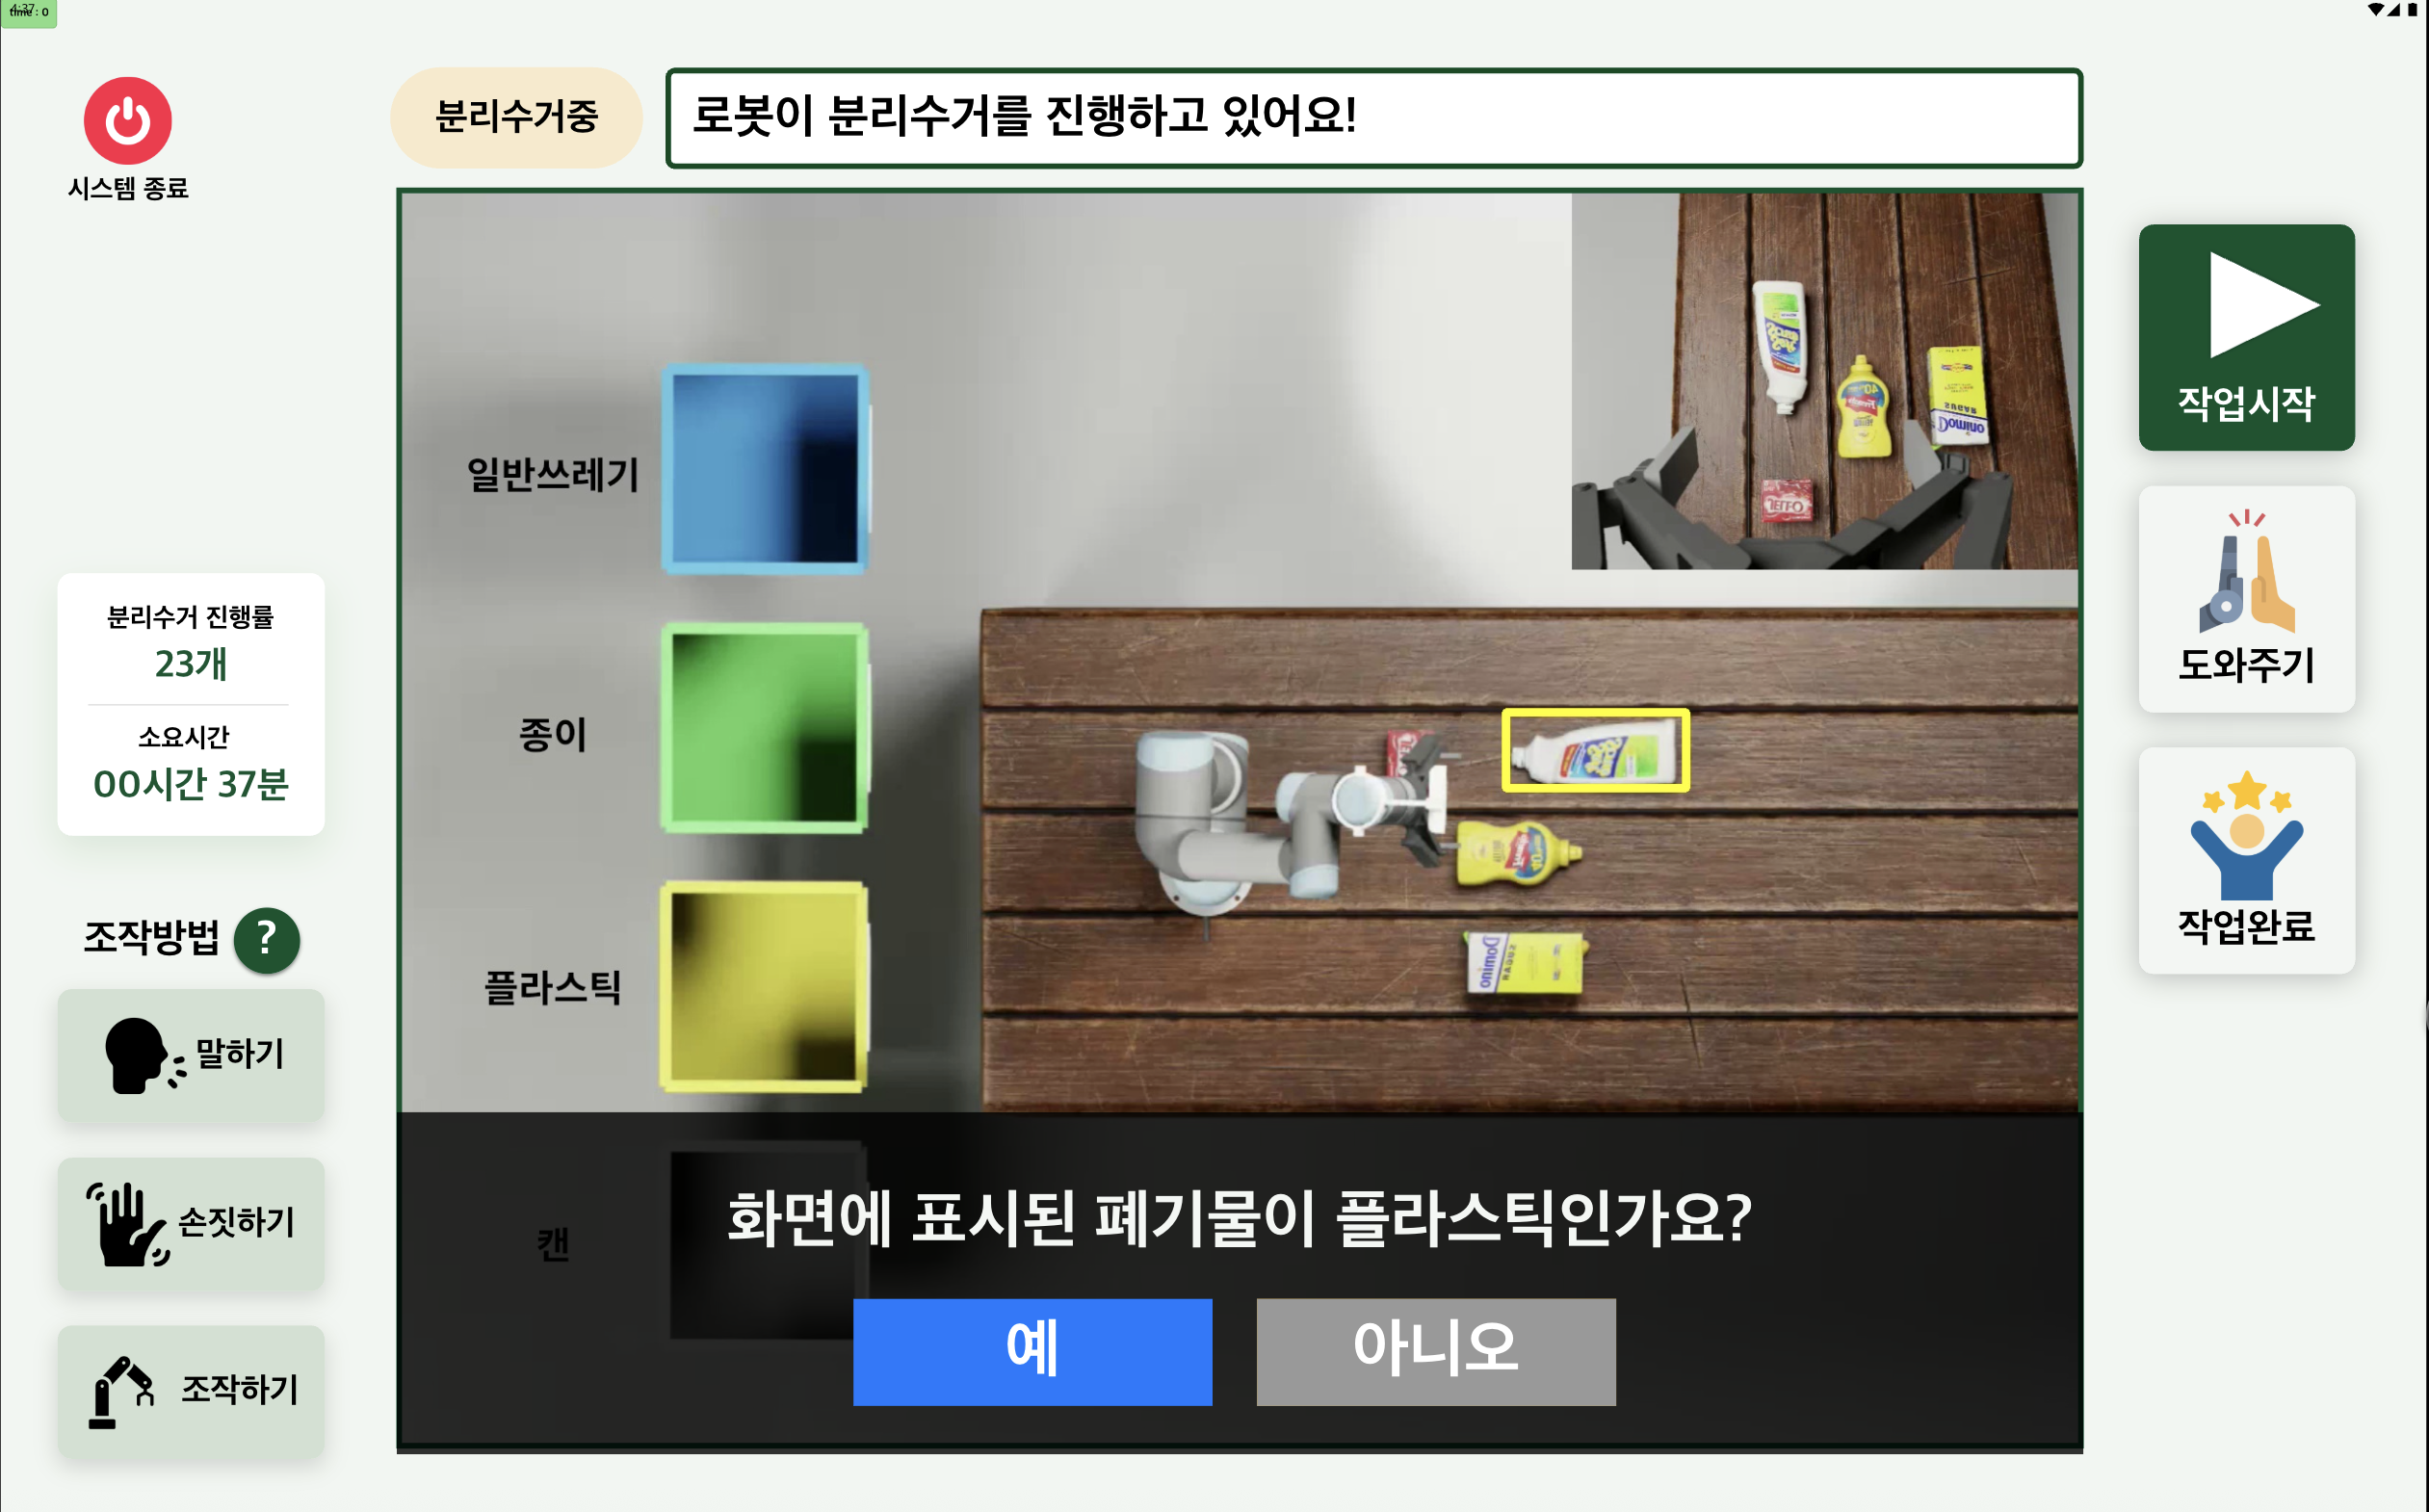
\includegraphics[width=\linewidth]{figures/fig_waste_our1.png}
        \caption{\textbf{Ours1} in waste sorting.}
        \label{fig:user_interface_waste_ours1}
    \end{subfigure}
    \hfill
    \begin{subfigure}[t]{0.32\textwidth}
        \centering
        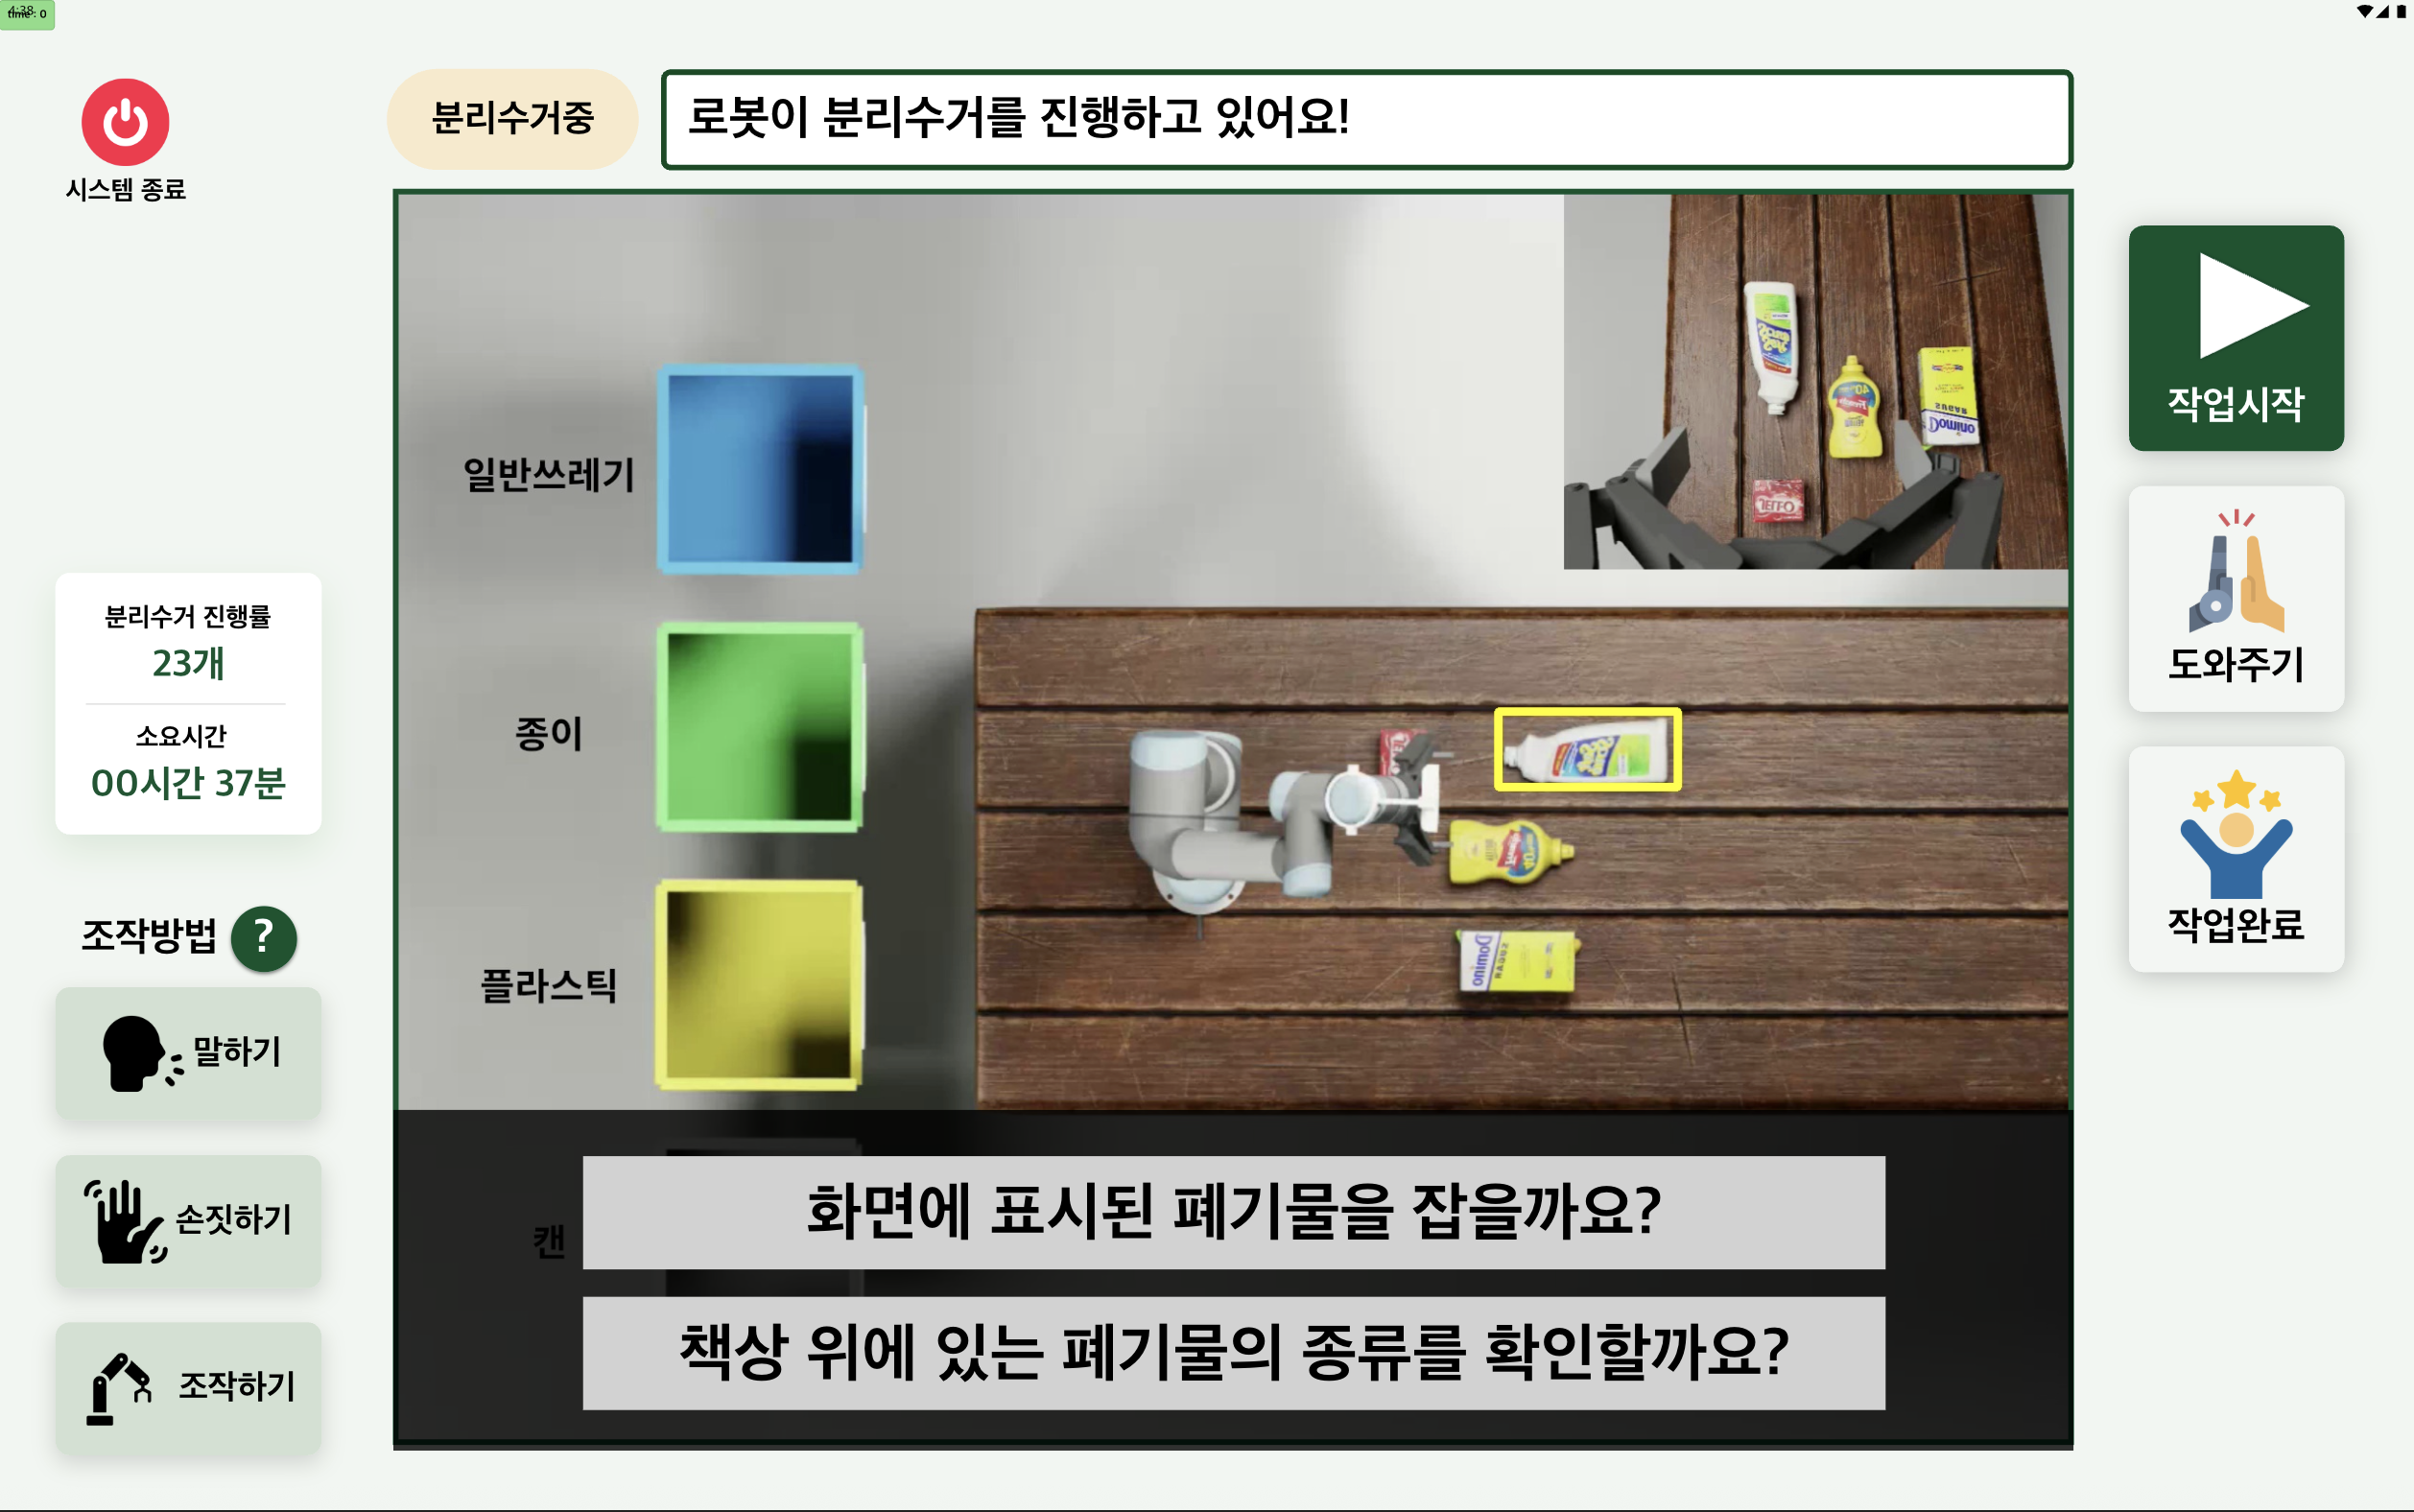
\includegraphics[width=\linewidth]{figures/fig_waste_knowno.png}
        \caption{\textbf{KnowNo} in waste sorting.}
        \label{fig:user_interface_waste_knowno}
    \end{subfigure}
    \hfill
    \begin{subfigure}[t]{0.32\textwidth}
        \centering
        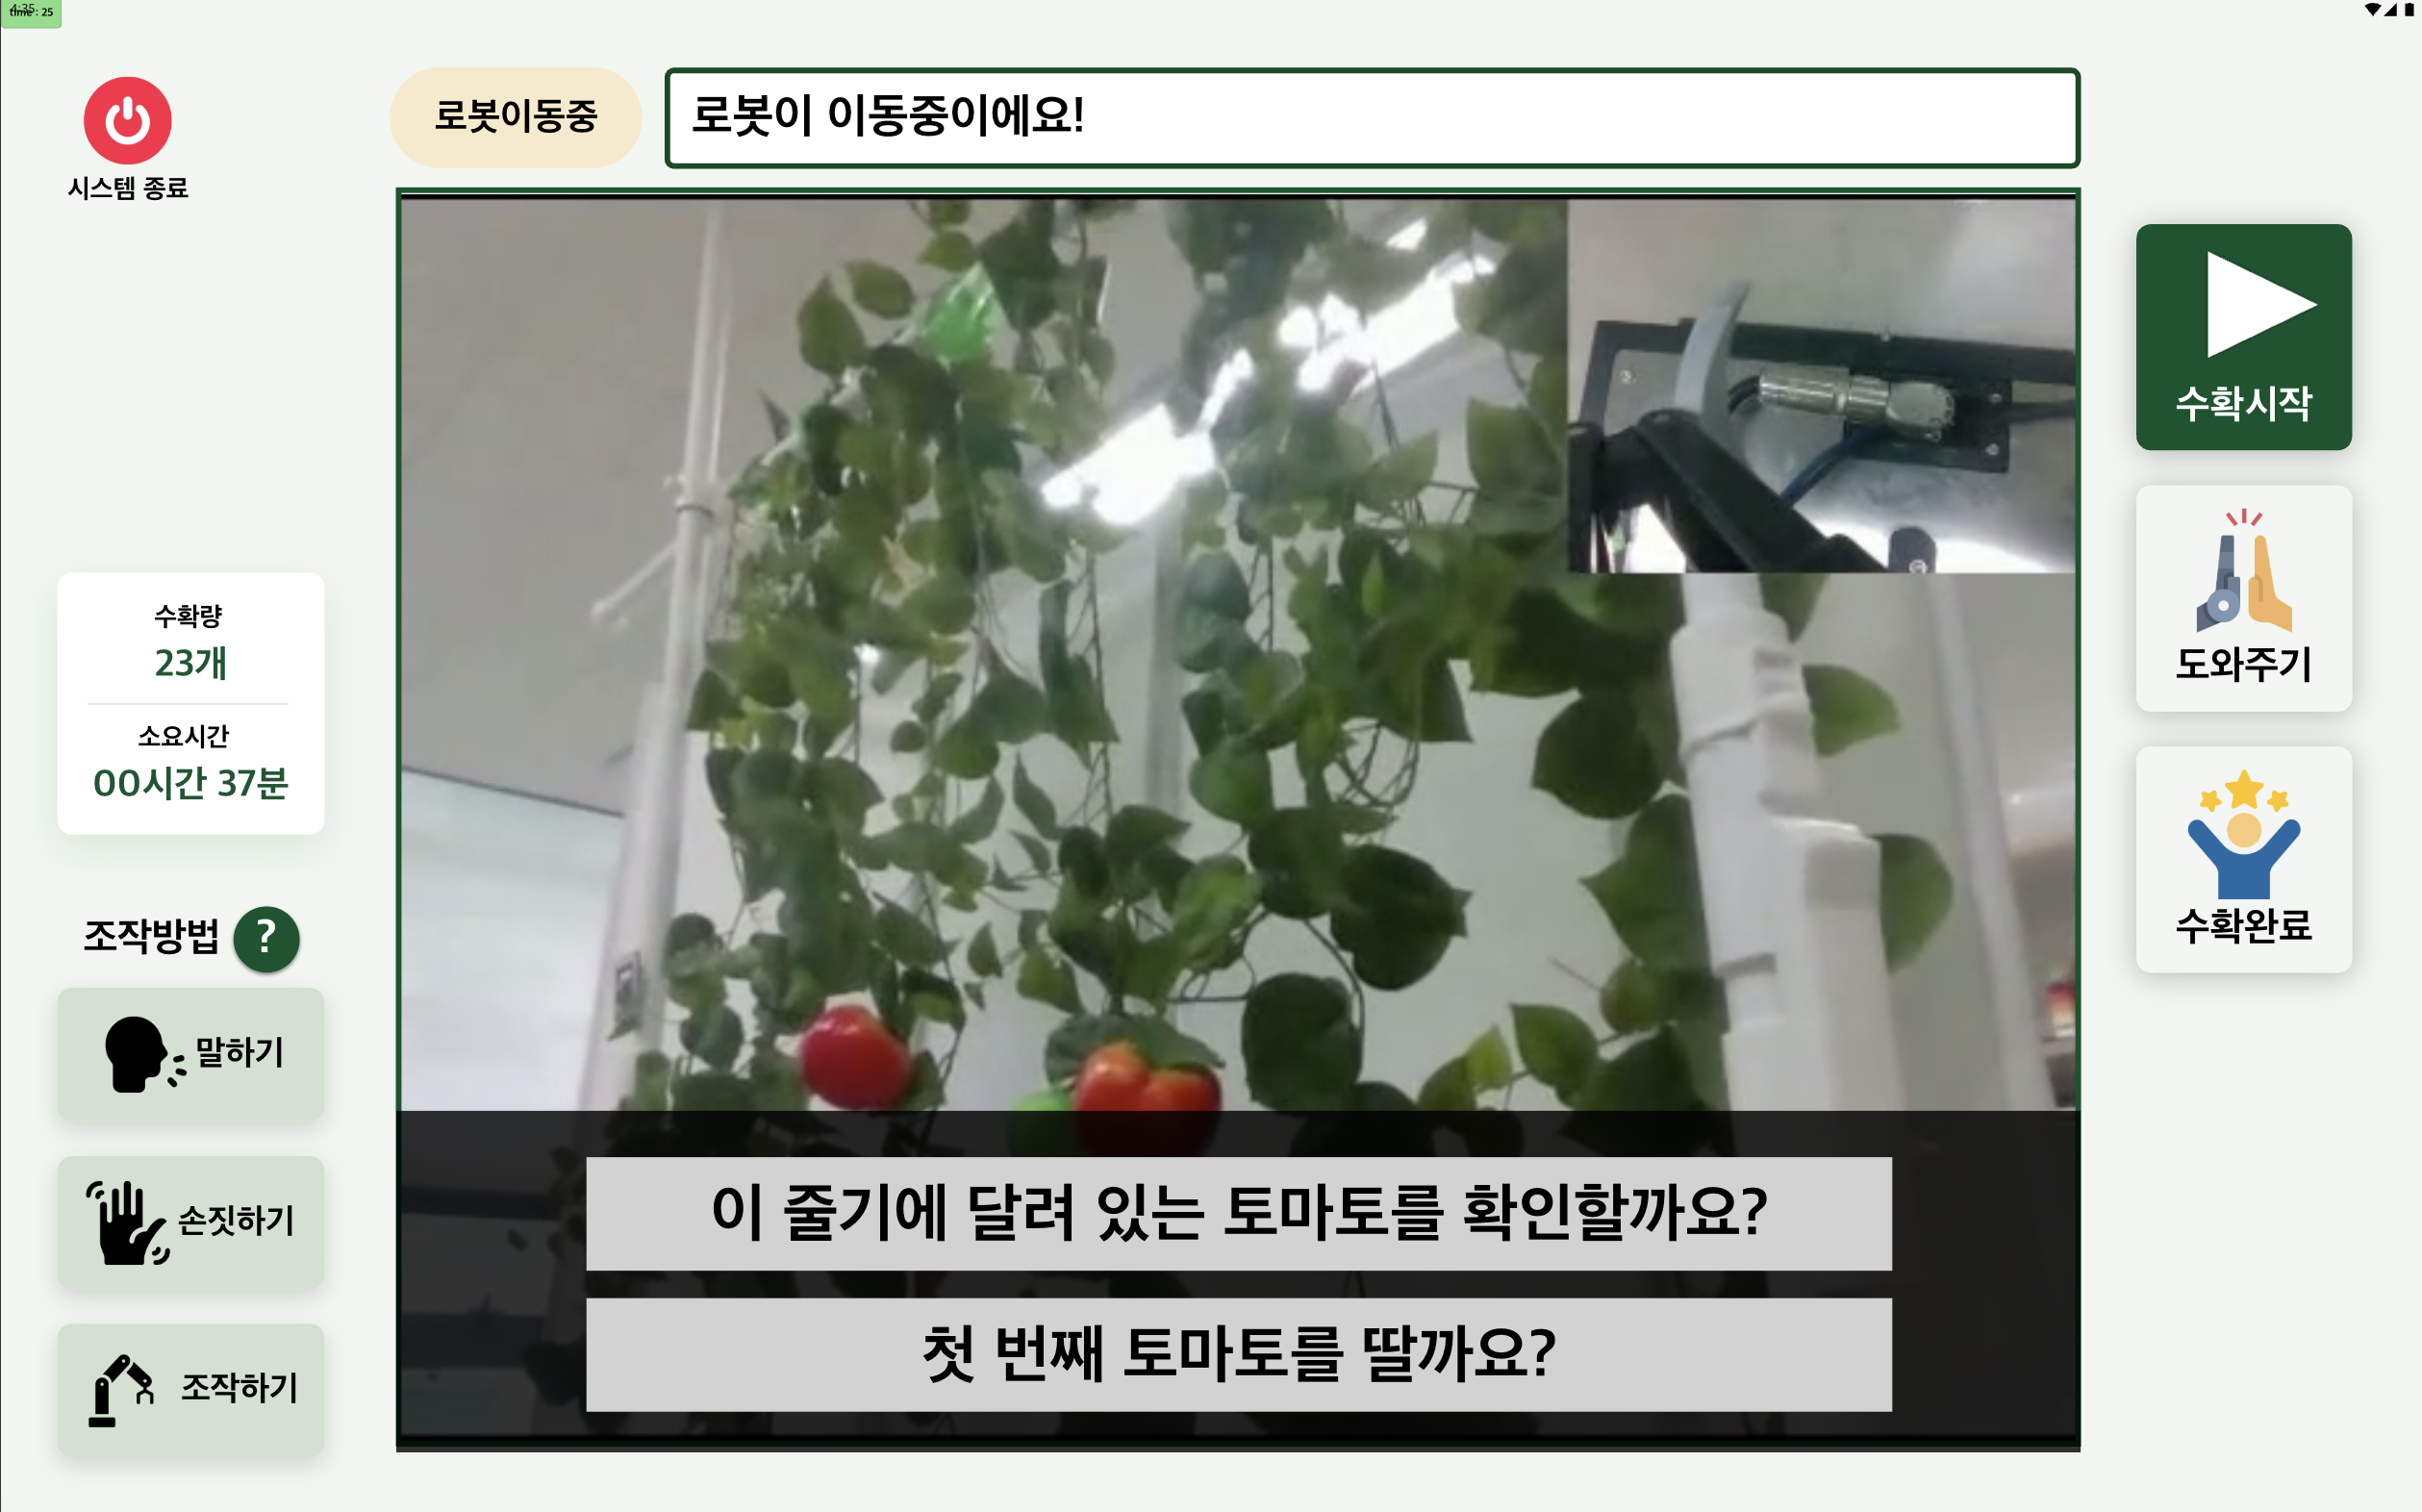
\includegraphics[width=\linewidth]{figures/fig_tomato_knowno.png}
        \caption{\textbf{KnowNo} in tomato harvesting.}
        \label{fig:user_interface_tomato_knowno}
    \end{subfigure}
    \caption{Representative user-study interfaces. In \textbf{Ours1}, users answer an observable task-level state question, such as whether the highlighted waste object is plastic. In \textbf{KnowNo}, users may be asked to choose a robot action, such as whether to grasp the displayed object or inspect the object category. This comparison contrasts state-level verification with action-level decision making.}
    \label{fig:user_interface_examples}
\end{figure*}

Before the experiment, participants received an explanation of the study objectives, the two task domains, and the robot interaction process. They were then introduced to the tablet interface and completed practice interactions to become familiar with the available information and response procedure. During the main session, participants completed ten trials without assistance. If a participant selected an incorrect answer, the response was recorded as incorrect for evaluation purposes, but the scenario continued using the intended task state so that subsequent interactions were not affected by earlier mistakes. After each scenario, participants completed questionnaires regarding workload, fatigue, and situation awareness. After all trials, participants provided qualitative feedback during a short debriefing session.

\subsubsection{Measures and Analysis}~\label{user:measures}

We analyzed the user study along four axes. First, task success measured whether participants provided all required responses correctly within a task. \textbf{No} was reported for questionnaire-based measures but omitted from task success because it contains no scorable user responses. Second, operation time measured the active user operation time after subtracting passive scenario video duration. \textbf{No} was also omitted from this analysis so that operation time reflects active interaction rather than the absence of interaction.

Third, subjective workload was measured using NASA Raw-TLX, and fatigue was measured using a self-reported fatigue item. Fourth, situation awareness was evaluated using SART and SAGAT-style questions. We further decomposed SAGAT into three levels: Lv1 measured perception of the current state, Lv2 measured comprehension of the task situation, and Lv3 measured projection of future task behavior.

For domain-level condition comparisons, we used Cochran's Q for binary task success and Friedman tests for continuous or ordinal measures. Post-hoc comparisons used exact McNemar tests for task success and exact Wilcoxon signed-rank tests for other measures, with Bonferroni correction. For SAGAT-level analysis, we compared Lv1, Lv2, and Lv3 within each domain--condition cell using Friedman tests and exact Wilcoxon signed-rank post-hoc tests with Bonferroni correction.

\subsubsection{Results: Task Success and Operation Time}~\label{user:results_task_time}

Table~\ref{tab:user_task_time} summarizes task success and operation time. In waste sorting, the condition effect on task success was significant, Cochran's $Q(3)=27.69$, $p<.001$, Kendall's $W=0.77$. \textbf{Ours1} achieved $91.7\%$ success and \textbf{Ours2} achieved $100.0\%$, matching or exceeding \textbf{All} ($91.7\%$). In contrast, \textbf{KnowNo} achieved only $8.3\%$. Post-hoc tests showed that \textbf{KnowNo} was significantly lower than \textbf{All} ($p=.012$), \textbf{Ours1} ($p=.012$), and \textbf{Ours2} ($p=.006$). In tomato harvesting, the condition effect was not significant, $Q(3)=5.40$, $p=.143$, but \textbf{Ours1} and \textbf{Ours2} both maintained $75.0\%$ success, compared with $66.7\%$ for \textbf{All}.

\begin{figure*}[t]
    \centering
    \begin{subfigure}[t]{0.24\textwidth}
        \centering
        
\includegraphics[width=\linewidth]{figures/waste_task_success.png}
        \caption{Waste success.}
        \label{fig:user_waste_task_success}
    \end{subfigure}
    \hfill
    \begin{subfigure}[t]{0.24\textwidth}
        \centering
        
\includegraphics[width=\linewidth]{figures/tomato_task_success.png}
        \caption{Tomato success.}
        \label{fig:user_tomato_task_success}
    \end{subfigure}
    \hfill
    \begin{subfigure}[t]{0.24\textwidth}
        \centering
        
\includegraphics[width=\linewidth]{figures/waste_operation_time.png}
        \caption{Waste operation time.}
        \label{fig:user_waste_operation_time}
    \end{subfigure}
    \hfill
    \begin{subfigure}[t]{0.24\textwidth}
        \centering
        
\includegraphics[width=\linewidth]{figures/tomato_operation_time.png}
        \caption{Tomato operation time.}
        \label{fig:user_tomato_operation_time}
    \end{subfigure}
    \caption{Task success and operation time across query strategies. \textbf{No} is omitted from these two analyses so the panels focus on scorable user responses and active user operation. Error bars indicate standard error; brackets mark Bonferroni-corrected significant post-hoc comparisons.}
    \label{fig:user_task_time_results}
\end{figure*}

\begin{table*}[t]
\centering
\caption{Task success and operation time by domain and condition. Values are mean $\pm$ standard error. \textbf{No} is omitted because these measures focus on scorable user responses and active user operation.}
\label{tab:user_task_time}
\small
\setlength{\tabcolsep}{5pt}
\begin{tabular*}{\textwidth}{@{\extracolsep{\fill}}llcccc}
\toprule
\textbf{Domain} & \textbf{Measure} & \textbf{All} & \textbf{Ours1} & \textbf{Ours2} & \textbf{KnowNo} \\
\midrule
Waste & Task success (\%) & $91.7 \pm 8.3$ & $91.7 \pm 8.3$ & $100.0 \pm 0.0$ & $8.3 \pm 8.3$ \\
Waste & Operation time (s) & $30.0 \pm 6.7$ & $11.2 \pm 1.4$ & $10.0 \pm 1.3$ & $29.2 \pm 5.7$ \\
Tomato & Task success (\%) & $66.7 \pm 14.2$ & $75.0 \pm 13.1$ & $75.0 \pm 13.1$ & $100.0 \pm 0.0$ \\
Tomato & Operation time (s) & $35.2 \pm 3.2$ & $21.4 \pm 3.5$ & $17.6 \pm 2.2$ & $25.9 \pm 5.4$ \\
\bottomrule
\end{tabular*}
\end{table*}

Operation time showed a similar pattern. In waste sorting, the condition effect was significant, $\chi^2(3)=15.61$, $p=.002$, $W=0.58$. \textbf{Ours1} ($11.2$~s) and \textbf{Ours2} ($10.0$~s) were much faster than \textbf{All} ($30.0$~s) and \textbf{KnowNo} ($29.2$~s). Post-hoc tests confirmed that both \textbf{Ours1} and \textbf{Ours2} were faster than \textbf{KnowNo} (both Bonferroni-adjusted $p=.023$). In tomato harvesting, the same direction was observed, with \textbf{Ours1} ($21.4$~s) and \textbf{Ours2} ($17.6$~s) faster than \textbf{All} ($35.2$~s), although the overall condition effect did not reach significance, $\chi^2(3)=6.57$, $p=.085$.

These results show that query content shaped interaction efficiency. In the waste sorting \textbf{KnowNo} interface, users saw the object and bounding box, but were asked to decide whether the robot should grasp the displayed object or inspect the waste category. This action-level decision required users to infer why the planner needed another detection action. By contrast, \textbf{Ours1} asked users to judge the observable state itself, such as whether the highlighted object was plastic. Users could answer this task-level question directly from the current visual evidence, resulting in high success and short operation time. Tomato harvesting produced a complementary pattern: the \textbf{KnowNo} condition reached $100.0\%$ task success because the tomato workflow made the next action more visually and temporally constrained after navigation, detection, picking, and scanning. Thus, action-level querying was easier to resolve in tomato harvesting than in waste sorting, where users had to decide whether hidden category uncertainty still justified another detect action.

\subsubsection{Results: Workload and Situation Awareness}~\label{user:results_workload_sa}

Table~\ref{tab:user_workload_sa} summarizes workload and SART. NASA-RTLX showed significant condition effects in both waste sorting, $\chi^2(4)=21.31$, $p<.001$, $W=0.44$, and tomato harvesting, $\chi^2(4)=16.31$, $p=.003$, $W=0.34$. In waste sorting, \textbf{Ours2} produced lower workload ($M=1.89$) than \textbf{KnowNo} ($M=2.54$; Bonferroni-adjusted $p=.010$). In tomato harvesting, \textbf{Ours1} ($M=1.89$) and \textbf{Ours2} ($M=1.81$) both reduced workload relative to \textbf{All} ($M=2.21$), with Bonferroni-adjusted $p=.020$ and $p=.039$, respectively. Fatigue did not show a significant condition effect, and SART did not differ significantly across conditions in either domain: waste, $\chi^2(4)=5.06$, $p=.281$; tomato, $\chi^2(4)=5.24$, $p=.264$.

\begin{figure*}[t]
    \centering
    \begin{subfigure}[t]{0.24\textwidth}
        \centering
        
\includegraphics[width=\linewidth]{figures/waste_nasa_rtlx.png}
        \caption{Waste NASA-RTLX.}
        \label{fig:user_waste_nasa}
    \end{subfigure}
    \hfill
    \begin{subfigure}[t]{0.24\textwidth}
        \centering
        
\includegraphics[width=\linewidth]{figures/tomato_nasa_rtlx.png}
        \caption{Tomato NASA-RTLX.}
        \label{fig:user_tomato_nasa}
    \end{subfigure}
    \hfill
    \begin{subfigure}[t]{0.24\textwidth}
        \centering
        
\includegraphics[width=\linewidth]{figures/waste_sart.png}
        \caption{Waste SART.}
        \label{fig:user_waste_sart}
    \end{subfigure}
    \hfill
    \begin{subfigure}[t]{0.24\textwidth}
        \centering
        
\includegraphics[width=\linewidth]{figures/tomato_sart.png}
        \caption{Tomato SART.}
        \label{fig:user_tomato_sart}
    \end{subfigure}
    \caption{Subjective workload and perceived situation awareness. NASA-RTLX is lower-is-better, whereas SART is higher-is-better. Error bars indicate standard error; brackets mark Bonferroni-corrected significant post-hoc comparisons.}
    \label{fig:user_workload_sart_results}
\end{figure*}

\begin{table*}[t]
\centering
\caption{Subjective workload and SART by domain and condition. Values are mean $\pm$ standard error. Lower NASA-RTLX indicates lower workload; higher SART indicates higher perceived situation awareness.}
\label{tab:user_workload_sa}
\small
\setlength{\tabcolsep}{4pt}
\begin{tabular*}{\textwidth}{@{\extracolsep{\fill}}llccccc}
\toprule
\textbf{Domain} & \textbf{Measure} & \textbf{All} & \textbf{No} & \textbf{Ours1} & \textbf{Ours2} & \textbf{KnowNo} \\
\midrule
Waste & NASA-RTLX & $2.06 \pm 0.24$ & $1.65 \pm 0.16$ & $2.26 \pm 0.28$ & $1.89 \pm 0.21$ & $2.54 \pm 0.29$ \\
Waste & SART & $3.11 \pm 0.21$ & $3.39 \pm 0.19$ & $3.41 \pm 0.18$ & $3.22 \pm 0.19$ & $3.35 \pm 0.23$ \\
Tomato & NASA-RTLX & $2.21 \pm 0.24$ & $1.72 \pm 0.19$ & $1.89 \pm 0.20$ & $1.81 \pm 0.15$ & $1.81 \pm 0.17$ \\
Tomato & SART & $3.26 \pm 0.25$ & $3.19 \pm 0.15$ & $3.10 \pm 0.24$ & $3.06 \pm 0.17$ & $3.02 \pm 0.23$ \\
\bottomrule
\end{tabular*}
\end{table*}

The workload and SART results show the main user-facing benefit of selective state queries: participants spent less active time and reported lower workload while retaining comparable perceived situation awareness. \textbf{Ours1} and \textbf{Ours2} therefore reduced interaction cost without drawing users away from the task state they needed to monitor.

\subsubsection{Results: SAGAT Levels}~\label{user:results_sagat_levels}

The SAGAT-level analysis provides a finer-grained view of how different query strategies shaped situation awareness. Table~\ref{tab:user_sagat_levels} reports Lv1, Lv2, and Lv3 accuracy for all conditions shown in the SAGAT level figures.

\begin{figure*}[t]
    \centering
    \begin{subfigure}[t]{0.19\textwidth}
        \centering
        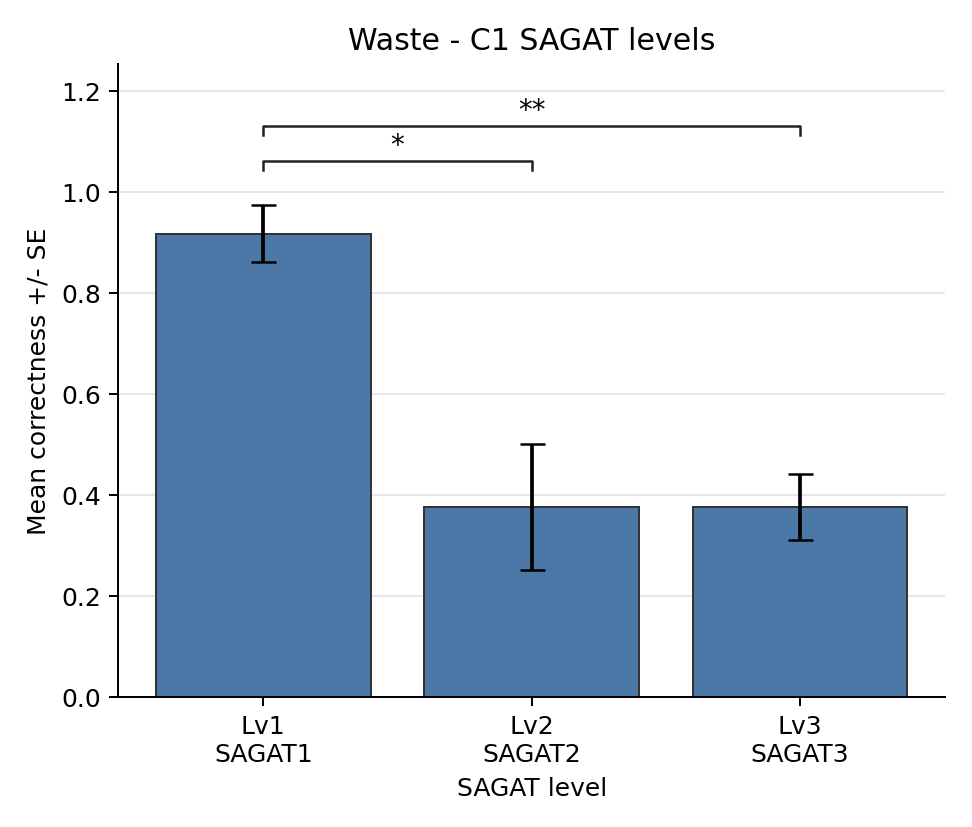
\includegraphics[width=\linewidth]{figures/waste_c1_sagat_levels.png}
        \caption{C1: All.}
    \end{subfigure}
    \hfill
    \begin{subfigure}[t]{0.19\textwidth}
        \centering
        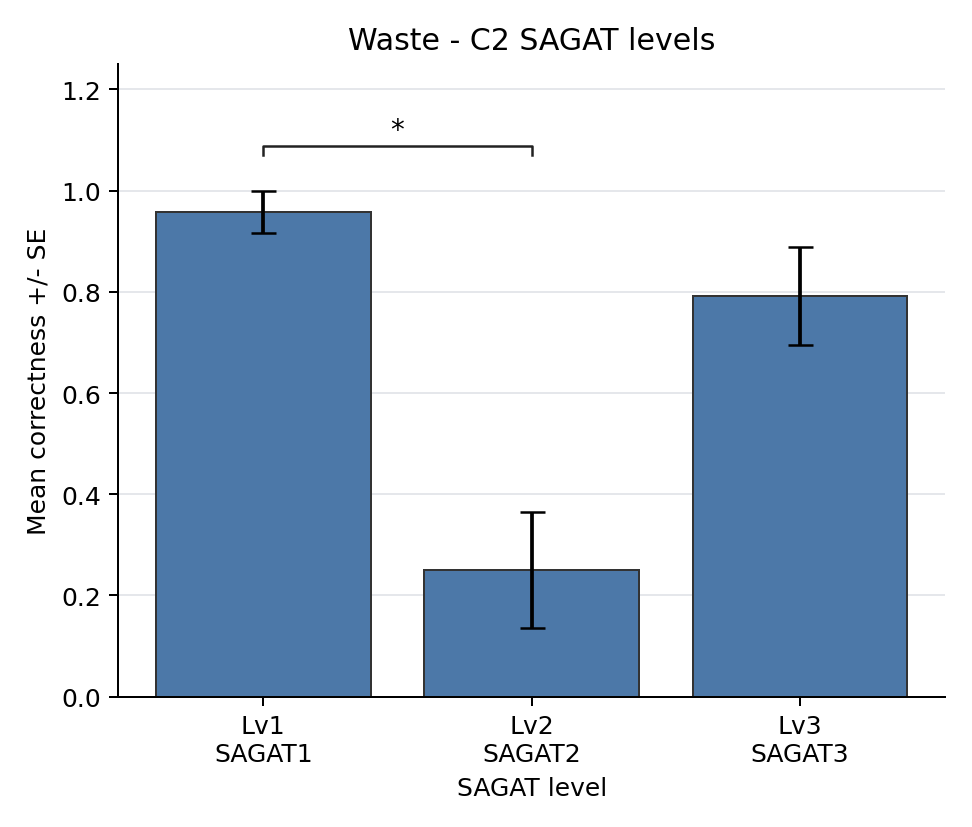
\includegraphics[width=\linewidth]{figures/waste_c2_sagat_levels.png}
        \caption{C2: No.}
    \end{subfigure}
    \hfill
    \begin{subfigure}[t]{0.19\textwidth}
        \centering
        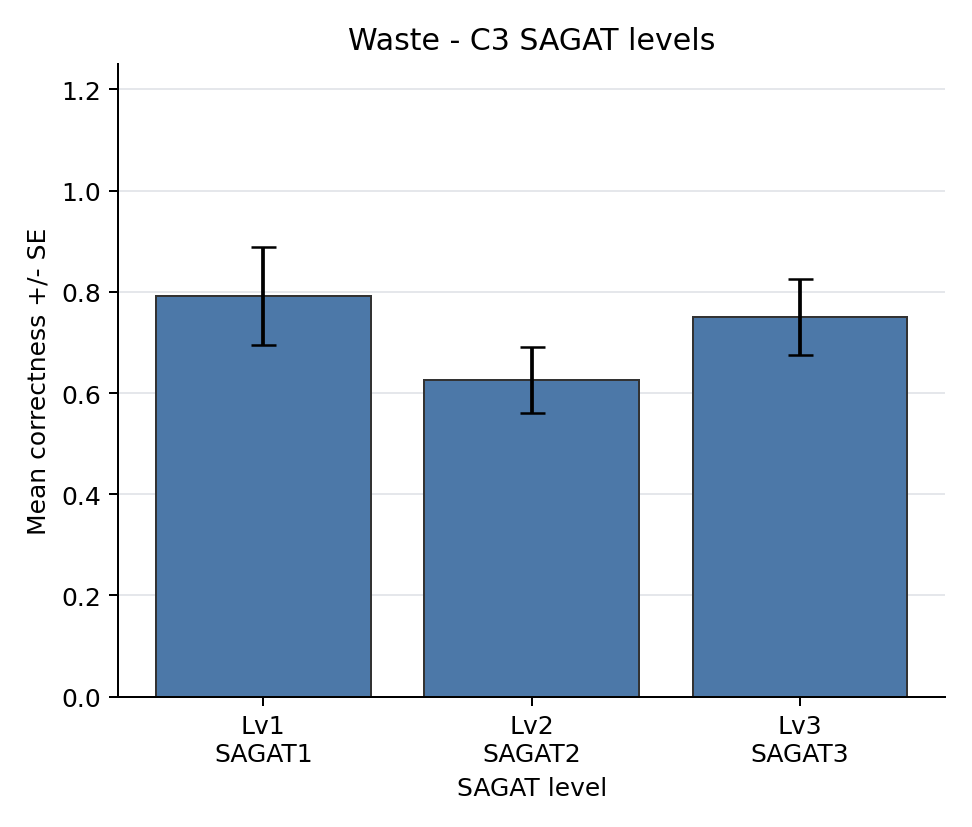
\includegraphics[width=\linewidth]{figures/waste_c3_sagat_levels.png}
        \caption{C3: Ours1.}
    \end{subfigure}
    \hfill
    \begin{subfigure}[t]{0.19\textwidth}
        \centering
        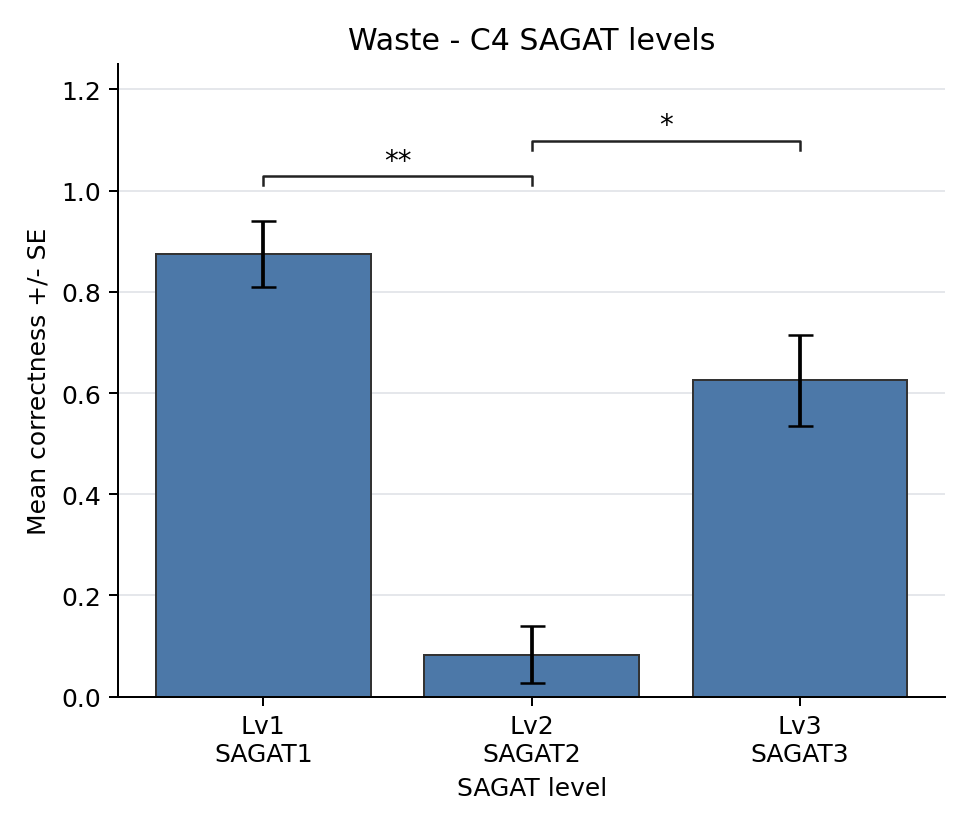
\includegraphics[width=\linewidth]{figures/waste_c4_sagat_levels.png}
        \caption{C4: Ours2.}
    \end{subfigure}
    \hfill
    \begin{subfigure}[t]{0.19\textwidth}
        \centering
        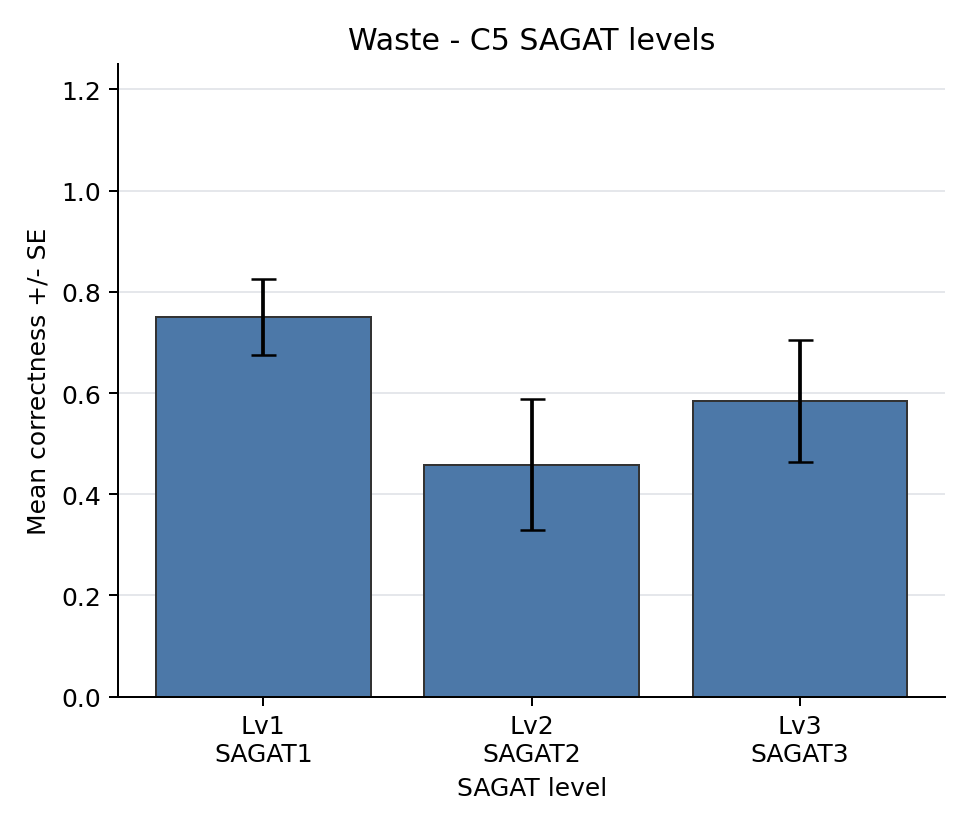
\includegraphics[width=\linewidth]{figures/waste_c5_sagat_levels.png}
        \caption{C5: KnowNo.}
    \end{subfigure}
    \caption{SAGAT level profiles in waste sorting. Each panel compares Lv1, Lv2, and Lv3 within a condition. Error bars indicate standard error; brackets mark Bonferroni-corrected significant post-hoc comparisons.}
    \label{fig:user_waste_sagat_levels}
\end{figure*}

\begin{figure*}[t]
    \centering
    \begin{subfigure}[t]{0.19\textwidth}
        \centering
        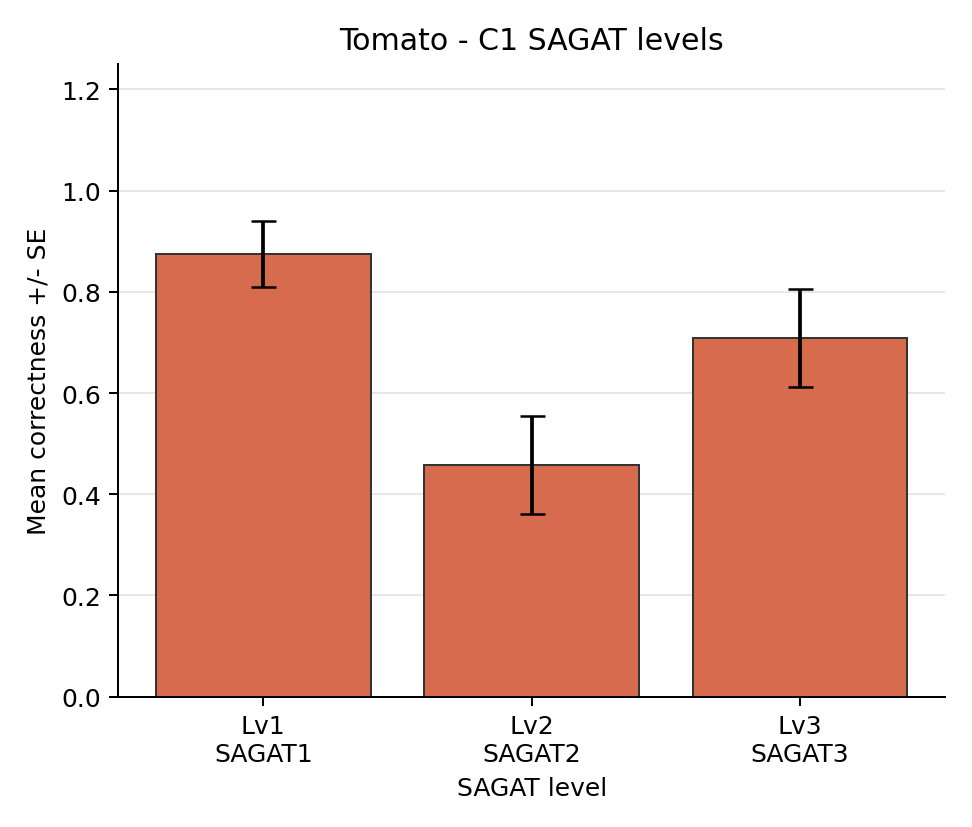
\includegraphics[width=\linewidth]{figures/tomato_c1_sagat_levels.png}
        \caption{C1: All.}
    \end{subfigure}
    \hfill
    \begin{subfigure}[t]{0.19\textwidth}
        \centering
        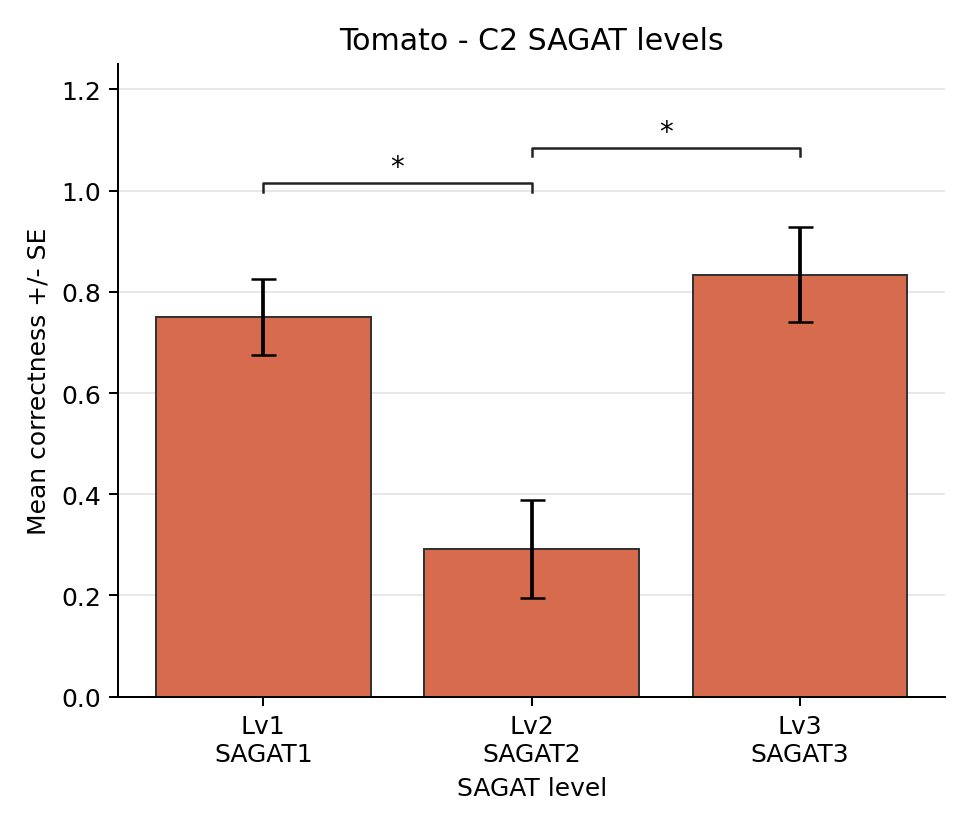
\includegraphics[width=\linewidth]{figures/tomato_c2_sagat_levels.png}
        \caption{C2: No.}
    \end{subfigure}
    \hfill
    \begin{subfigure}[t]{0.19\textwidth}
        \centering
        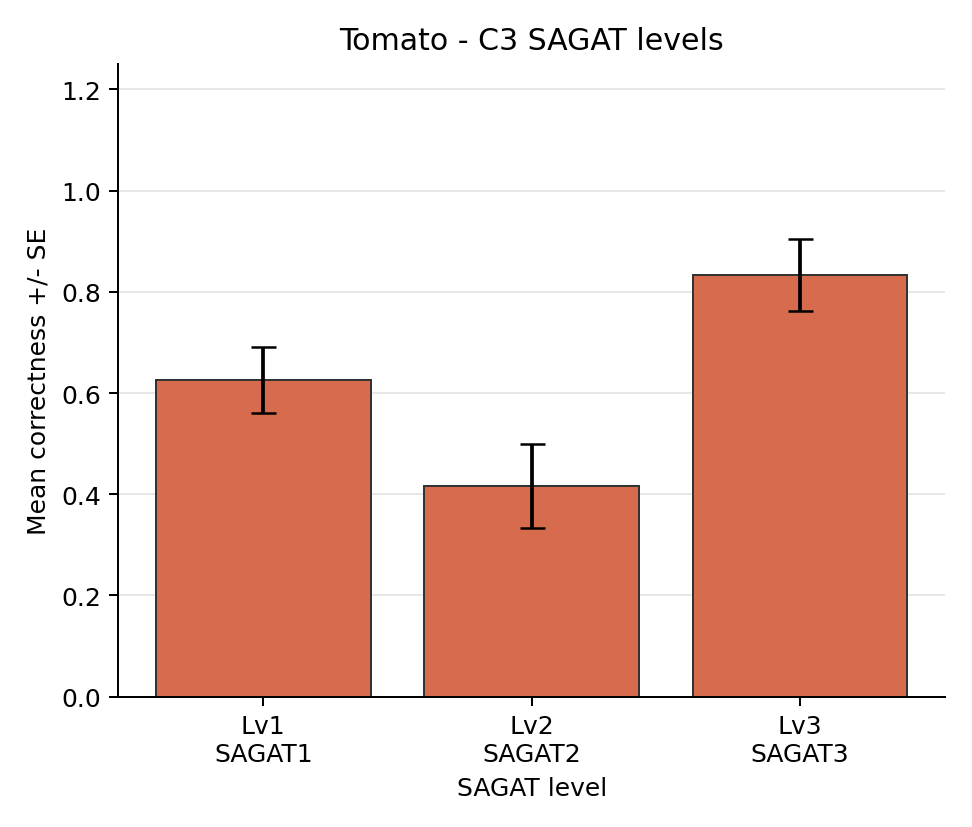
\includegraphics[width=\linewidth]{figures/tomato_c3_sagat_levels.png}
        \caption{C3: Ours1.}
    \end{subfigure}
    \hfill
    \begin{subfigure}[t]{0.19\textwidth}
        \centering
        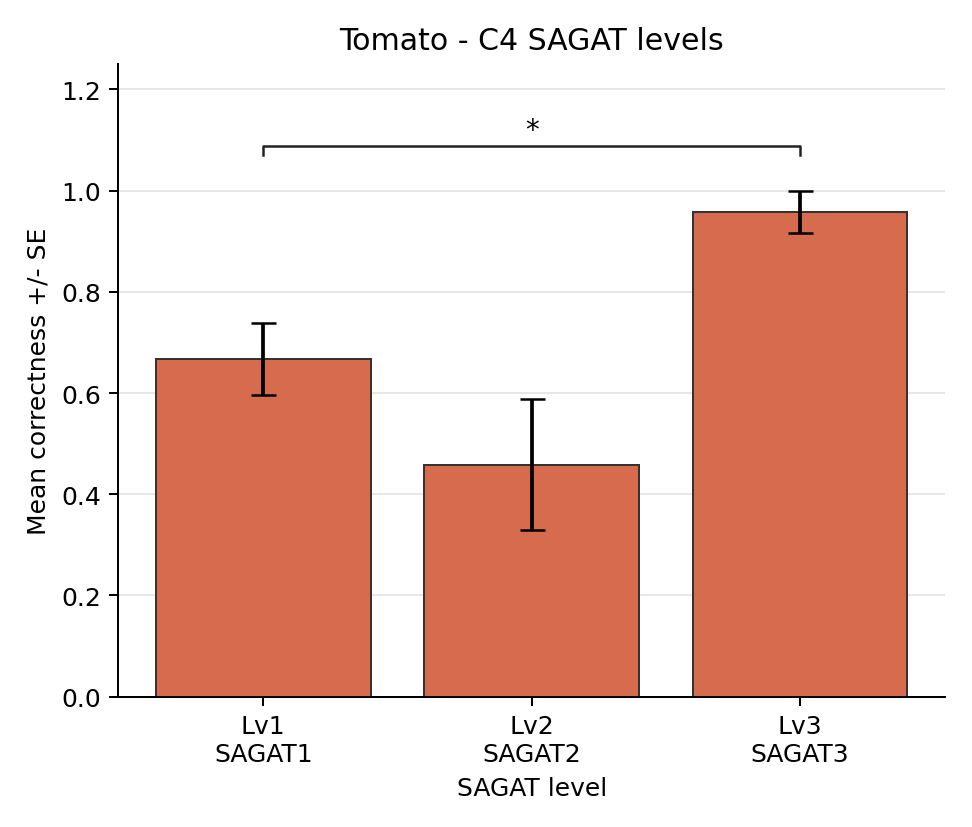
\includegraphics[width=\linewidth]{figures/tomato_c4_sagat_levels.png}
        \caption{C4: Ours2.}
    \end{subfigure}
    \hfill
    \begin{subfigure}[t]{0.19\textwidth}
        \centering
        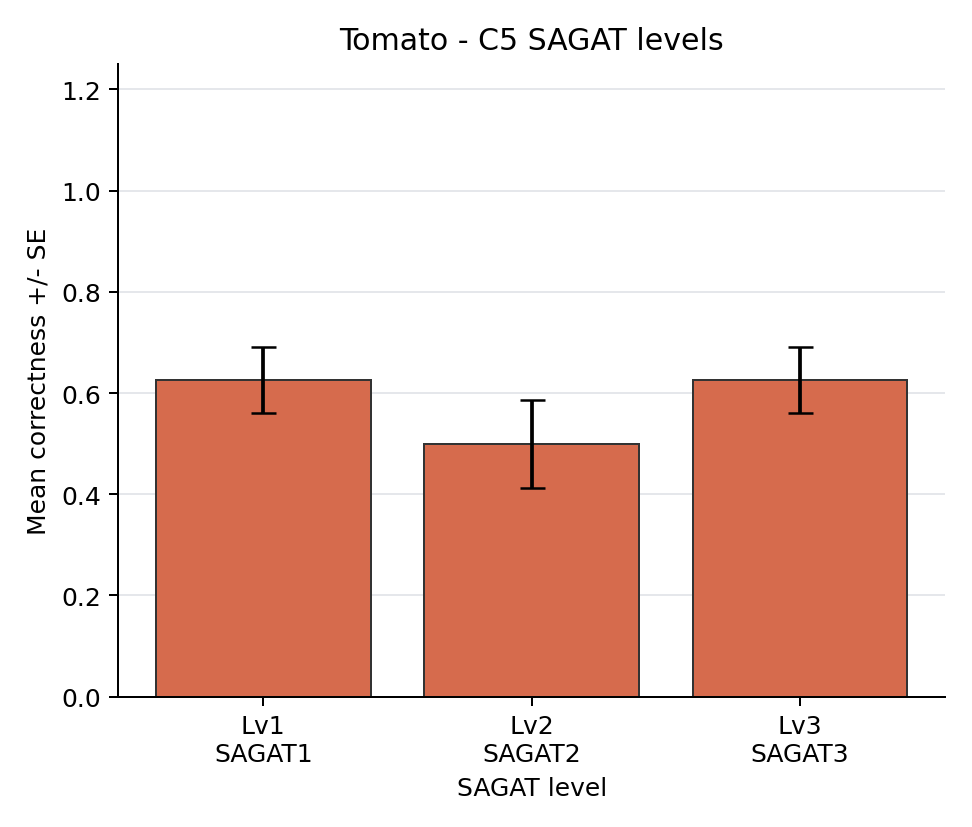
\includegraphics[width=\linewidth]{figures/tomato_c5_sagat_levels.png}
        \caption{C5: KnowNo.}
    \end{subfigure}
    \caption{SAGAT level profiles in tomato harvesting. Each panel compares Lv1, Lv2, and Lv3 within a condition. Error bars indicate standard error; brackets mark Bonferroni-corrected significant post-hoc comparisons.}
    \label{fig:user_tomato_sagat_levels}
\end{figure*}

\begin{table*}[t]
\centering
\caption{SAGAT level accuracy by domain and condition. Values are mean $\pm$ standard error. Lv1, Lv2, and Lv3 correspond to perception, comprehension, and projection, respectively.}
\label{tab:user_sagat_levels}
\small
\setlength{\tabcolsep}{4pt}
\begin{tabular*}{\textwidth}{@{\extracolsep{\fill}}llccc}
\toprule
\textbf{Domain} & \textbf{Condition} & \textbf{Lv1} & \textbf{Lv2} & \textbf{Lv3} \\
\midrule
Waste & All & $0.92 \pm 0.06$ & $0.38 \pm 0.13$ & $0.38 \pm 0.07$ \\
Waste & No & $0.96 \pm 0.04$ & $0.25 \pm 0.12$ & $0.79 \pm 0.10$ \\
Waste & Ours1 & $0.79 \pm 0.10$ & $0.63 \pm 0.07$ & $0.75 \pm 0.08$ \\
Waste & Ours2 & $0.88 \pm 0.07$ & $0.08 \pm 0.06$ & $0.63 \pm 0.09$ \\
Waste & KnowNo & $0.75 \pm 0.08$ & $0.46 \pm 0.13$ & $0.58 \pm 0.12$ \\
\midrule
Tomato & All & $0.88 \pm 0.07$ & $0.46 \pm 0.10$ & $0.71 \pm 0.10$ \\
Tomato & No & $0.75 \pm 0.08$ & $0.29 \pm 0.10$ & $0.83 \pm 0.09$ \\
Tomato & Ours1 & $0.63 \pm 0.07$ & $0.42 \pm 0.08$ & $0.83 \pm 0.07$ \\
Tomato & Ours2 & $0.67 \pm 0.07$ & $0.46 \pm 0.13$ & $0.96 \pm 0.04$ \\
Tomato & KnowNo & $0.63 \pm 0.07$ & $0.50 \pm 0.09$ & $0.63 \pm 0.07$ \\
\bottomrule
\end{tabular*}
\end{table*}

In waste sorting, \textbf{All} produced high Lv1 accuracy ($M=0.92$), while Lv2 and Lv3 were lower ($M=0.38$ for both). This profile reflects strong awareness of visible information under continuous supervision. In contrast, \textbf{Ours1} maintained a more balanced profile across Lv1, Lv2, and Lv3 ($0.79$, $0.63$, and $0.75$), suggesting that state-level uncertainty queries supported not only perception but also task comprehension and projection.

\textbf{Ours2} showed a more specialized profile. In waste sorting, it kept Lv1 high ($0.88$) and Lv3 relatively high ($0.63$), while Lv2 was low ($0.08$), indicating that broader query exposure emphasized visible state recognition and future task tracking more than intermediate causal explanations of why a specific query was issued. In tomato harvesting, Lv3 reached $0.96$, the highest value among all tomato conditions. The difference between Lv1 and Lv3 in tomato \textbf{Ours2} was significant after Bonferroni correction ($p=.047$). Thus, the two proposed variants produced different forms of situation awareness: \textbf{Ours1} supported a more balanced awareness profile, whereas \textbf{Ours2} particularly strengthened projection of future task behavior.

\subsubsection{Discussion}~\label{user:discussion}

The user-study results highlight a central design point: effective selective querying depends on matching the query to information users can judge from the interface. \textbf{Ours1} and \textbf{Ours2} used state-level questions grounded in observable task facts, supporting high success with shorter operation time and lower workload. \textbf{KnowNo} asked action-level questions, which shifted the interaction toward planner-state inference. In waste sorting, this placed the key decision on detect-versus-grasp selection when the visual scene looked actionable but the planner still needed category evidence.

The \textbf{KnowNo} cases also clarify the role of transparency. Visual highlights and scene views are useful when they align with the decision users are asked to make. In waste sorting, the \textbf{KnowNo} display showed the object and its bounding box, making the object salient without directly revealing the planner's category uncertainty. State-level queries align the visual cue and requested judgment more directly: the interface highlights the object, and the question asks users to verify the task fact associated with that object.

The SAGAT results further show that query strategies shape the structure of situation awareness. \textbf{Ours1} produced relatively balanced Lv1--Lv3 performance, supporting both current-state understanding and future-action projection. \textbf{Ours2}, especially in tomato harvesting, produced high Lv3 accuracy, suggesting that its broader query distribution encouraged users to follow the overall task flow. These patterns imply that situation awareness is not determined only by how much information is shown; it also depends on what kind of question the system asks.

Overall, effective selective querying is a design strategy for placing human attention at belief-relevant moments. A useful query is grounded in information that users can interpret from the interface while still being informative for the robot's planner. When this alignment holds, human feedback improves task performance, reduces cognitive burden, and shapes situation awareness in a task-relevant way.

The present user study provides a controlled first evaluation with $12$ participants in a narrow age range of 21--26 years. This setting allowed us to compare all conditions within participant and keep scenario timing consistent across query policies. A natural next step is to run the same query policies in fully autonomous long-horizon deployments with broader participant groups.
